\section{Problem 2}

\subsection{Question}
\vspace*{10pt}
Download the TimeMaps for each of the target URIs.  We'll use the ODU Memento Aggregator, so for example:\\
\\
URI-R = http://www.cs.odu.edu/\\
\\
URI-T = http://mementoproxy.cs.odu.edu/aggr/timemap/link/1/http://www.cs.odu.edu/\\
\\
Create a histogram* of URIs vs. number of Mementos (as computed from
the TimeMaps).  For example, 100 URIs with 0 Mementos, 300 URIs
with 1 Memento, 400 URIs with 2 Mementos, etc.\\
\\
* = https://en.wikipedia.org/wiki/Histogram
\subsection{Answer}
The python script in Listing \ref{listing:memfind} was used to retrieve the timemaps and then parse the returned html, traveling down the rabbit hole if the target URI has more than 1000 mementos.
\vspace{1mm}
\lstinputlisting[language=Python, caption={mementofinder.py}, label=listing:memfind]{q2/mementofinder.py}

\vspace{5mm}
The dataset created Listing \ref{listing:memfind}. A log scale was used along the y-axis to show more detail among the results. The script in Listing \ref{listing:bld_hist} was used to create the histogram in Figure \ref{fig:hist_ss}, which shows the distribution of mementos per site from the dataset of Question 1.
\vspace{2mm}
\lstinputlisting[language=R, caption={build\_histogram.r}, label=listing:bld_hist]{q2/build_histogram.r}
\vspace{2mm}
\lstinputlisting[caption=Sample of Memento Links, linerange=7-27]
{q2/site_mementos.txt}
\vspace*{5pt}
\begin{figure}[h]
\centering
\fbox{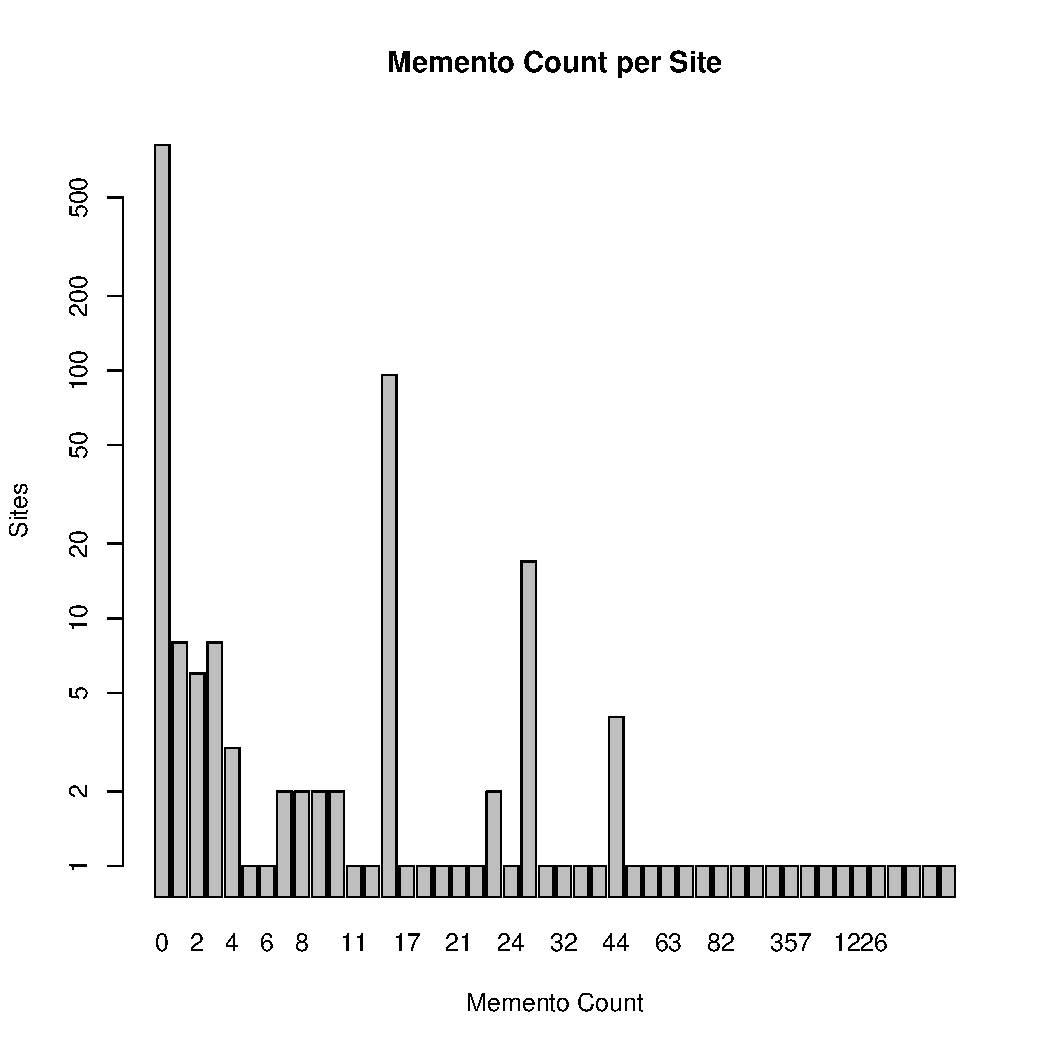
\includegraphics[scale=.85]{q2/histogram.pdf}}
\caption{Histogram of Site Mementos}
\label{fig:hist_ss}
\end{figure}
